%!TEX root = ../thesis.tex

\section{提案手法の概要}
本研究では, 従来手法をベースに「直進」, 「左折」, 「右折」の目標とする進行方向の情報(以下, 「目標方向」と称する)をデータセットと学習器へ追加する. これにより, 訓練済みの学習器の出力を用いた走行において, 目標方向により任意の経路を選択可能とする機能の追加を行った. なお, 追加した要素以外は従来手法と同様である. 提案手法全体の流れを\figref{Fig:suggest_work}に示す. 

\begin{figure}[hbtp]
     \centering
    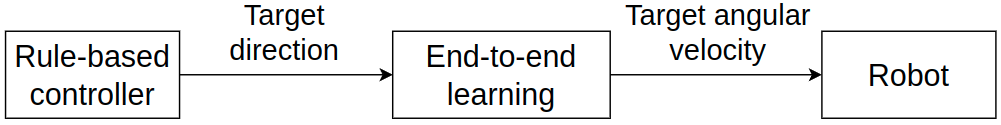
\includegraphics[keepaspectratio, scale=0.38]
         {images/suggest_work.png}
    \caption{Overall flow of the proposed method}
    \label{Fig:suggest_work}
\end{figure}

最終的にはカメラ画像を入力として, トポロジカルマップによって生成される目標方向に従って, 目的地まで移動する自律走行の手法を提案することを検討する. トポロジカルマップとは\figref{Fig:tsudanuma}に示すように, 分岐路などの目印(ノード)とつながり(エッジ)を持つ簡略化された地図である.

% \vspace{0.5cm}
\newpage

\vspace{0.5cm}

\begin{figure}[hbtp]
     \centering
    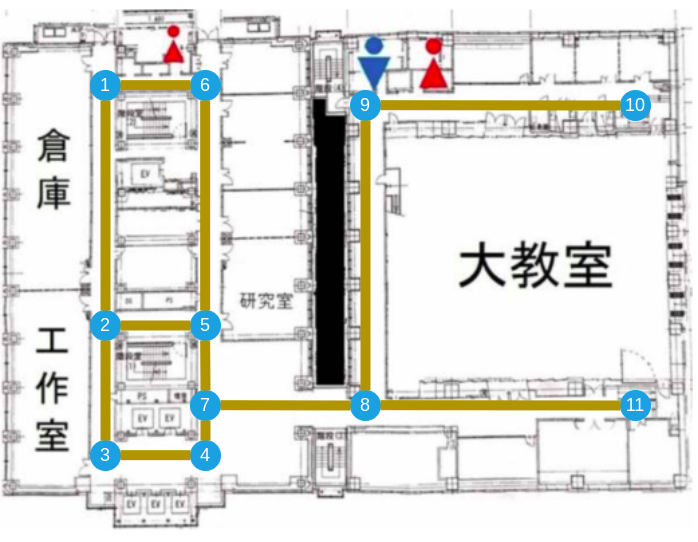
\includegraphics[keepaspectratio, scale=0.45]
         {images/tsudanuma.png}
    \caption{Topological map}
    \label{Fig:tsudanuma}
\end{figure}

% 従来手法で用いていたデータセットと学習器の入力へ, 「直進」「左折」などの目標方向を追加する. これにより, 学習器の出力による自律移動において, 経路を選択する機能の追加を行った. なお, 追加した要素以外は従来手法と同様である.

% \subsection{RoboCup}

% \begin{figure}[hbtp]
%   \centering
%  \includegraphics[keepaspectratio, scale=0.4]
%       {images/deeplearning_model.png}
%  \caption{Neural network}
%  \label{Fig:Neural network}
% \end{figure}

% \subsubsection{etc...}

\newpage
